%! TEX root = ./main.tex

\newpage

\section{Introduction}

\subsection{Background}

In the context of global climate change, forest management strategies are an effective way to achieve carbon sequestration and sink enhancement. Forests have multiple economic, ecological, and cultural functions and are the key link between the natural environment and the development of human society.\cite{LalR} By studying the changes of forest carbon sequestration(Figure 1), we can deduce the changes of natural succession and socio-economic conditions, which is of great practical significance.

However, previous forest carbon sequestration strategies are mostly based on the carbon sequestration of forests themselves\cite{landsat7,urbanforest}  , and the carbon sequestration associated with forest products is often neglected. Studies\cite{WoodProducts}  have shown that forest products have significant carbon sequestration capacity and emission reduction potential over their life cycle. Therefore, the carbon sequestration of forest products and regenerated forests resulting from wood harvesting should be integrated into the forest carbon sequestration system for a comprehensive assessment to derive more reasonable forest management measures including harvesting cycle and harvesting scale.

Moreover, the objectives of forest management measures should not be limited to ecological and economic goals, but also the socio-cultural functions of forests should not be ignored. 

Thus, an universal forest valuation system is in need to provide comprehensive assessment and guidance for forest management measures. At the same time, it is necessary to popularize this system, raise public awareness of ecological environment, and guide the public to actively participate in forestry and ecological construction with practical actions in order to couple a healthy and sustainable social-economic-natural composite ecosystem and achieve long-term development.
\begin{figure}[htp]
    \centering
    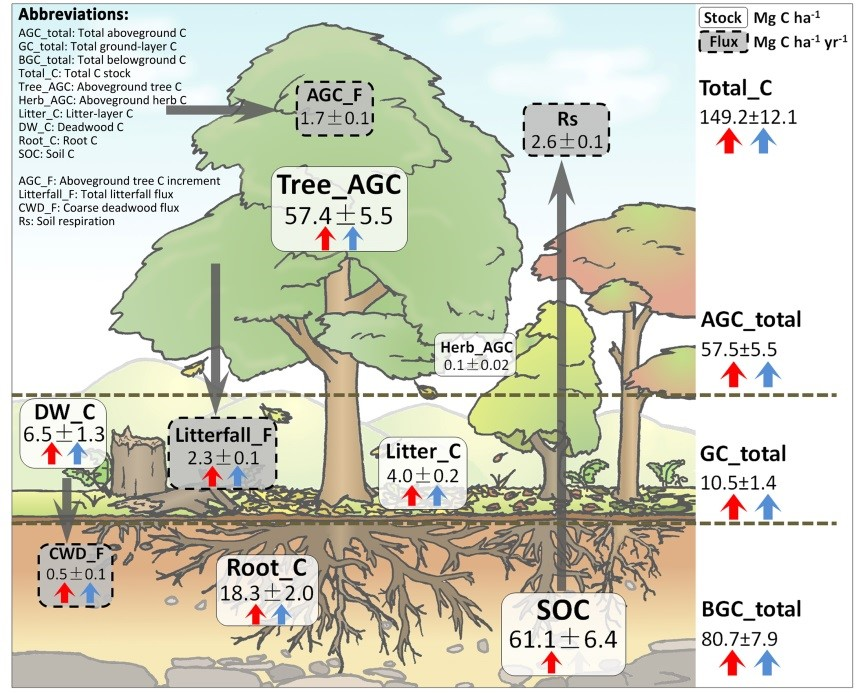
\includegraphics[width=13cm]{figs/carbon_cycle.jpg}
    \caption{Forest carbon cycle.}
    \label{fig:my_label}
\end{figure}

\subsection{Our work}
First, we developed a carbon sequestration model using the biomass method. We decomposed the objectives into two parts: carbon sequestration by forest products and carbon sequestration by forests. Management options (including cutting strategy and product strategy) were introduced into the model as an intermediate link between the two. 

We derived the best calculation function for forest biomass by curve fitting, and converted biomass into carbon sequestration based on relevant research. Forest products are broadly classified into three types of raw materials using cluster analysis for forest product carbon sequestration calculation. Combining the final destinations of trees and forest products (death, landfill and incineration), the amount of forest carbon sequestration was calculated. By analyzing the changes in carbon sequestration under different management scenarios, we can derive the amount of forest carbon sequestration under specified scenarios for reference of forest management measures.
The specific model is shown in Figure 2.(Task1)

Next, we use the entropy weight method to make a comprehensive evaluation of forest values. Combining carbon sequestration models and related research bases, indicators are constructed from three traditional dimensions of ecology, society and economy to reflect the comprehensive value of forests. We also introduce sustainability variables as a reference for forest development potential, taking into account the current green development trend.
The specific model is shown in Figure 3.(Task2)

Thirdly, we take a planted test forest in Qingping state-owned forest in Hunan Province as an example and substitute it into the model to study the best management plan. A 2 × 9 management plan matrix was obtained by setting different cutting rates and different product management strategies. We use the maximum value of the weighted sum of the factors as the objective function and program MATLAB to implement the model solution to obtain the best management plan under comprehensive evaluation.

Based on the existing management plan of this forest, we calculated the amount of carbon sequestered in the current forest over a 100-year period. Comparing the best management strategy and the existing management strategy, the transition plan of the two scenarios is derived. (Task3)

Finally, we performed a sensitivity analysis of the model with the results of the example calculations and explained and analyzed the strengths and limitations of the model. The results of the study are finally presented to the public in the form of a short non-technical article. We explain the design logic of the model in relatively easy-to-understand language to justify the forest management measures derived from the model that contradict conventional wisdom. The article \emph {More logging, more fixed carbon? Reasonable!} is presented.(Task4)


